\begin{frame}\frametitle{Total and Differential Cross Section}
\begin{figure}[htb]
  \begin{center}
   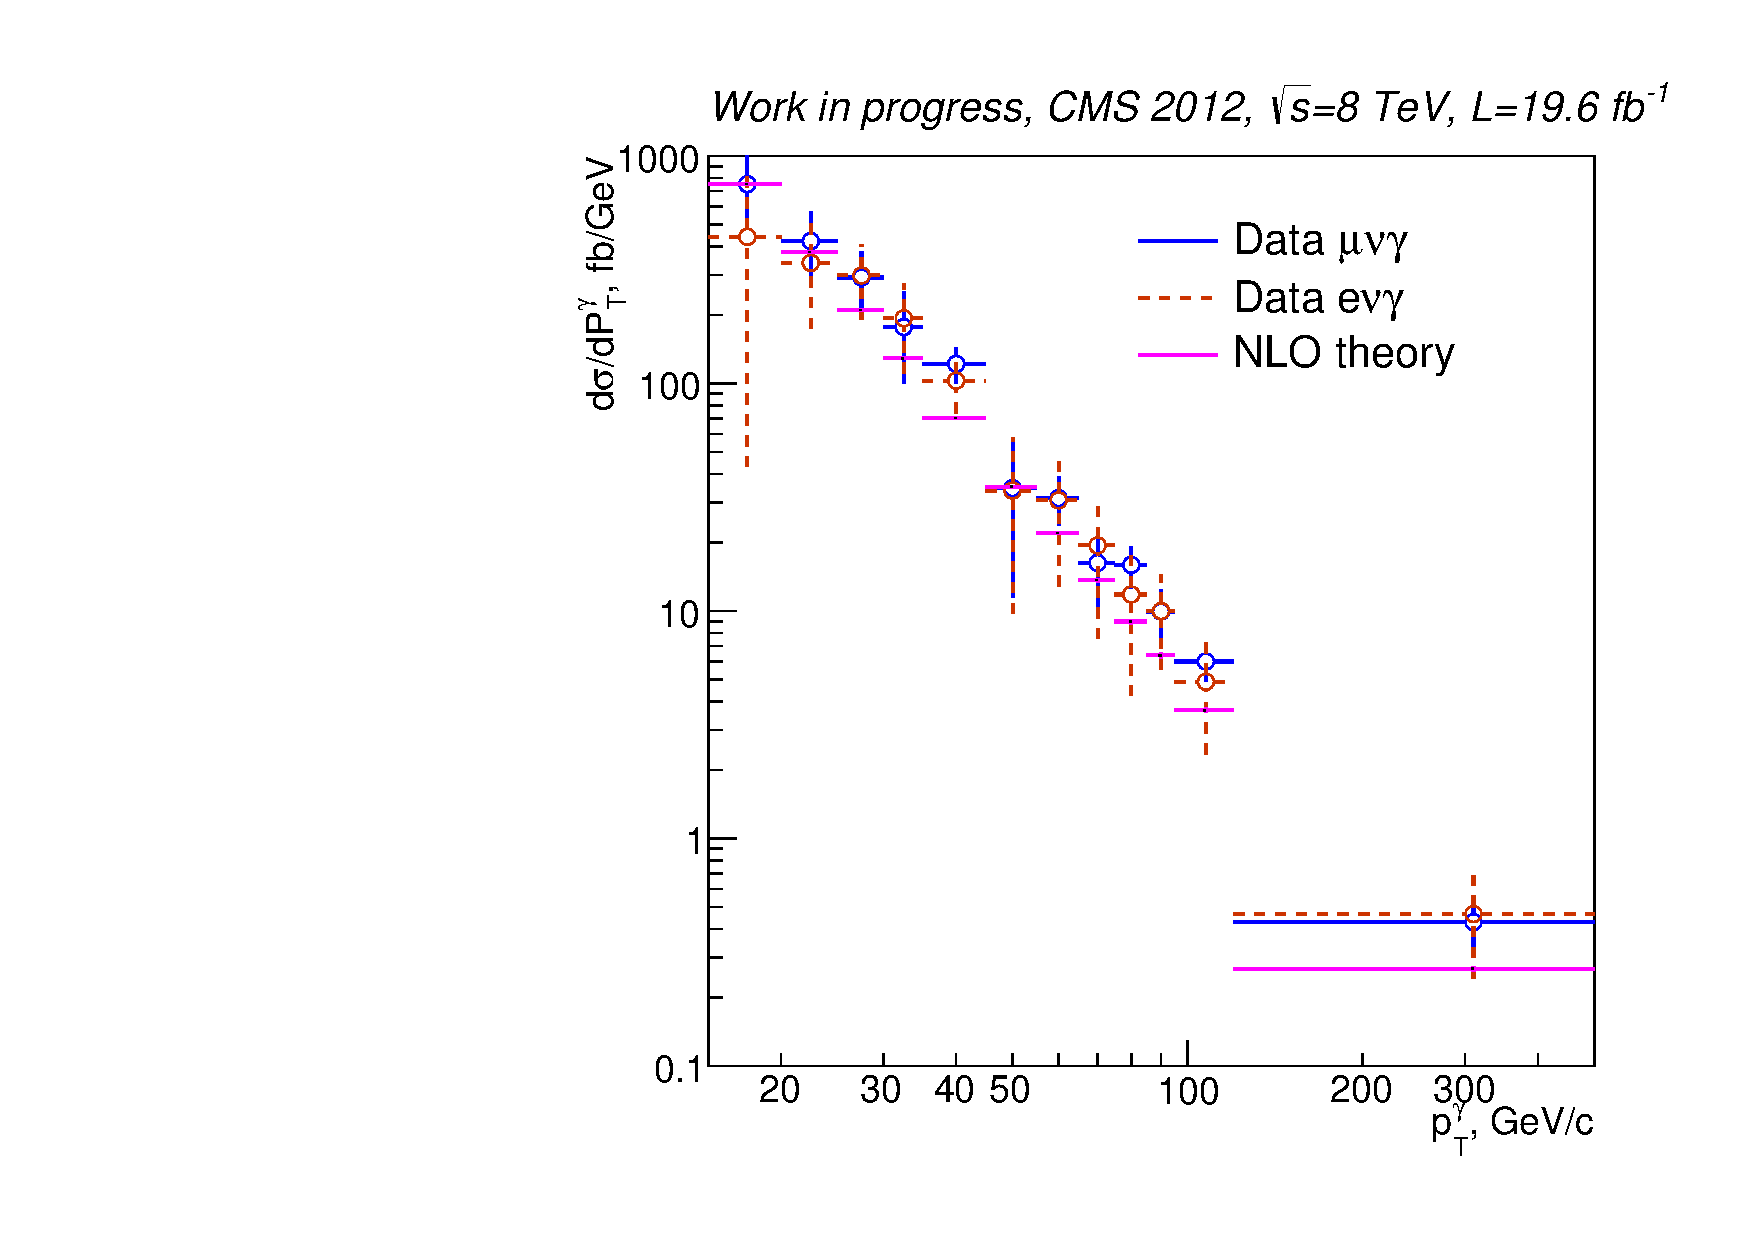
\includegraphics[width=0.5\textwidth]{../figs/figs_v11/ChannelsMERGED_WGamma/CrossSection/compareCSWGamma.pdf}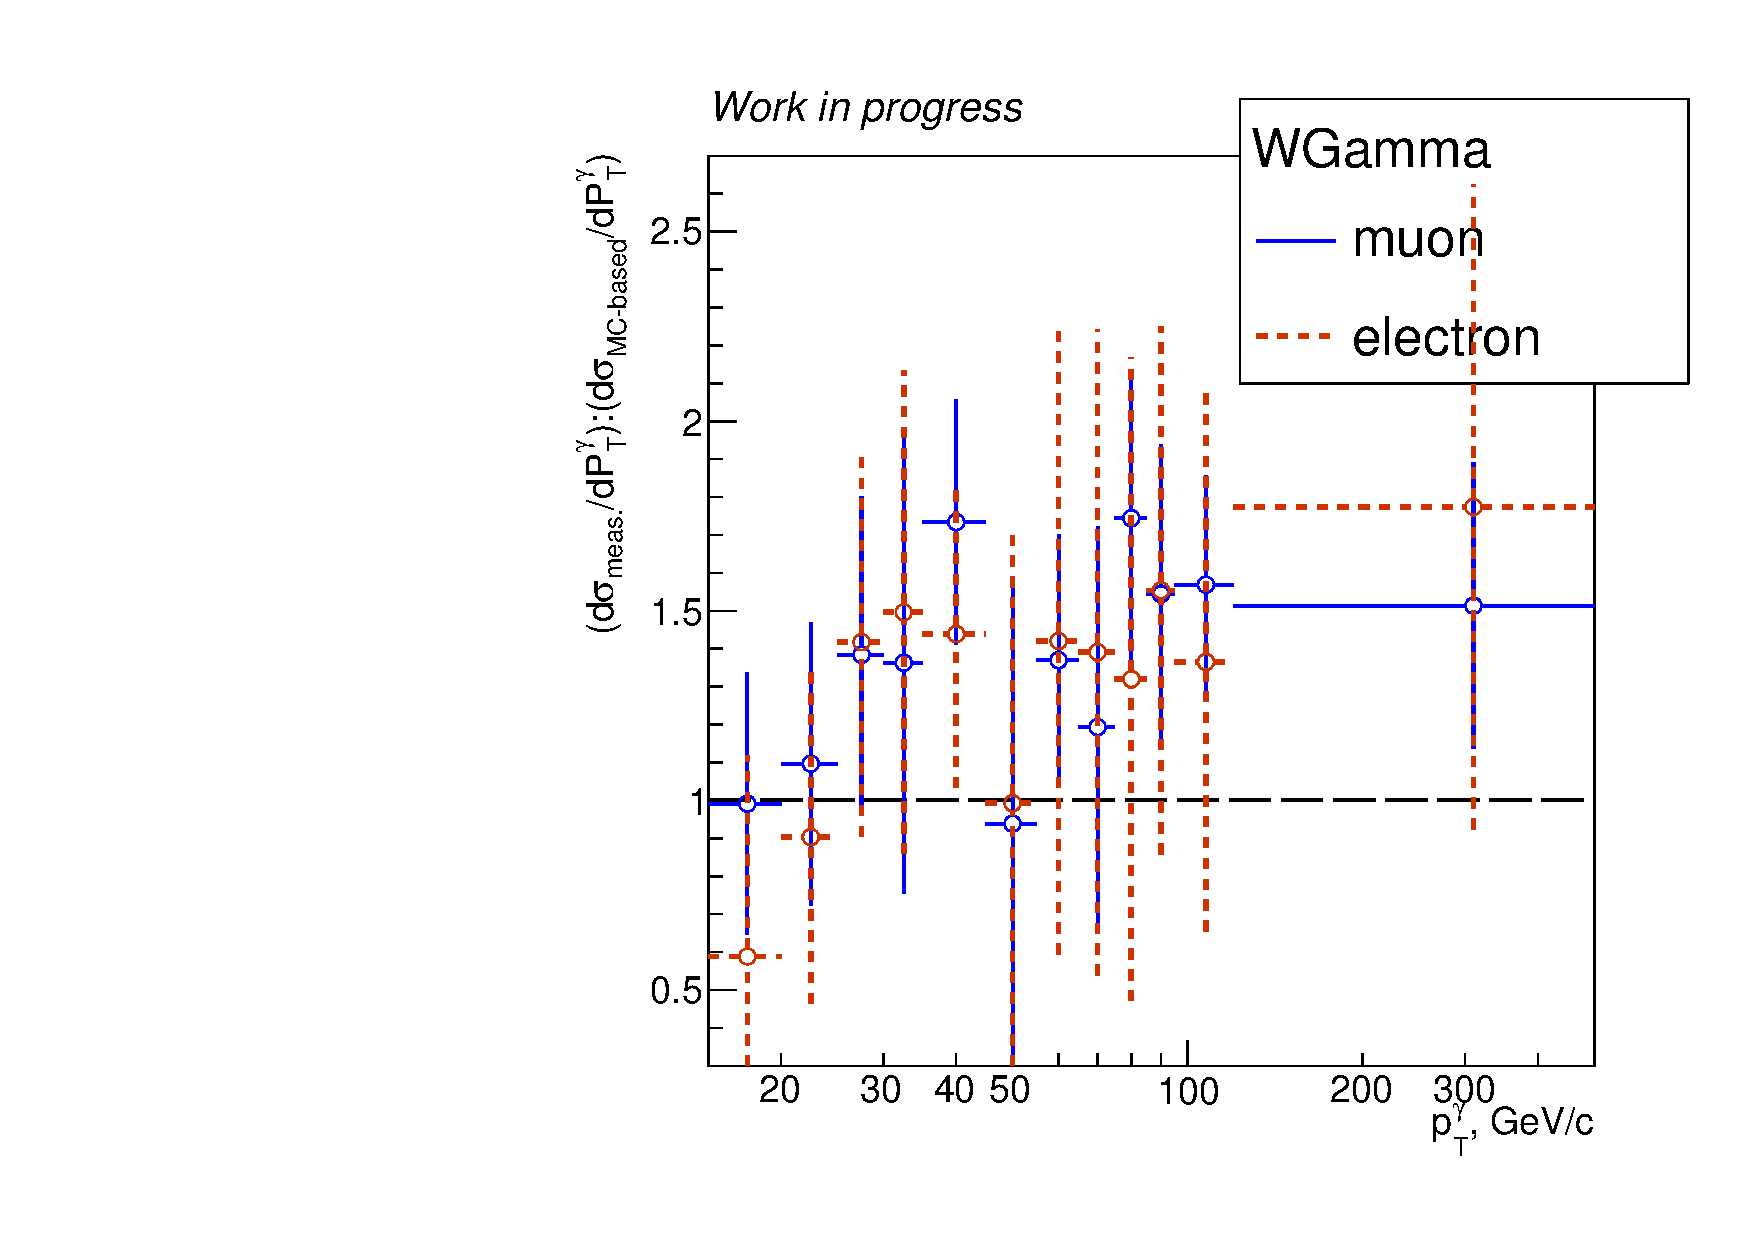
\includegraphics[width=0.5\textwidth]{../figs/figs_v11/ChannelsMERGED_WGamma/CrossSection/compareCSratioTheoryWGamma.pdf}\\
  \end{center}
\end{figure}
\scriptsize
{\bfseries{Total cross section ($P_T^{\gamma}>15$~GeV):}}\\
MC-based: $\sigma=9101$~fb\\
Measured, muon channel:   $\sigma = 10949 \pm 91 \pm 1463$~fb\\
Measured, electron channel:   $\sigma = 9146 \pm 185 \pm 2213$~fb\\
\end{frame}%{Differential Cross Section. Plots}

\begin{frame}\frametitle{ZGamma check. Differential Cross Section}
\begin{figure}[htb]
  \begin{center}
 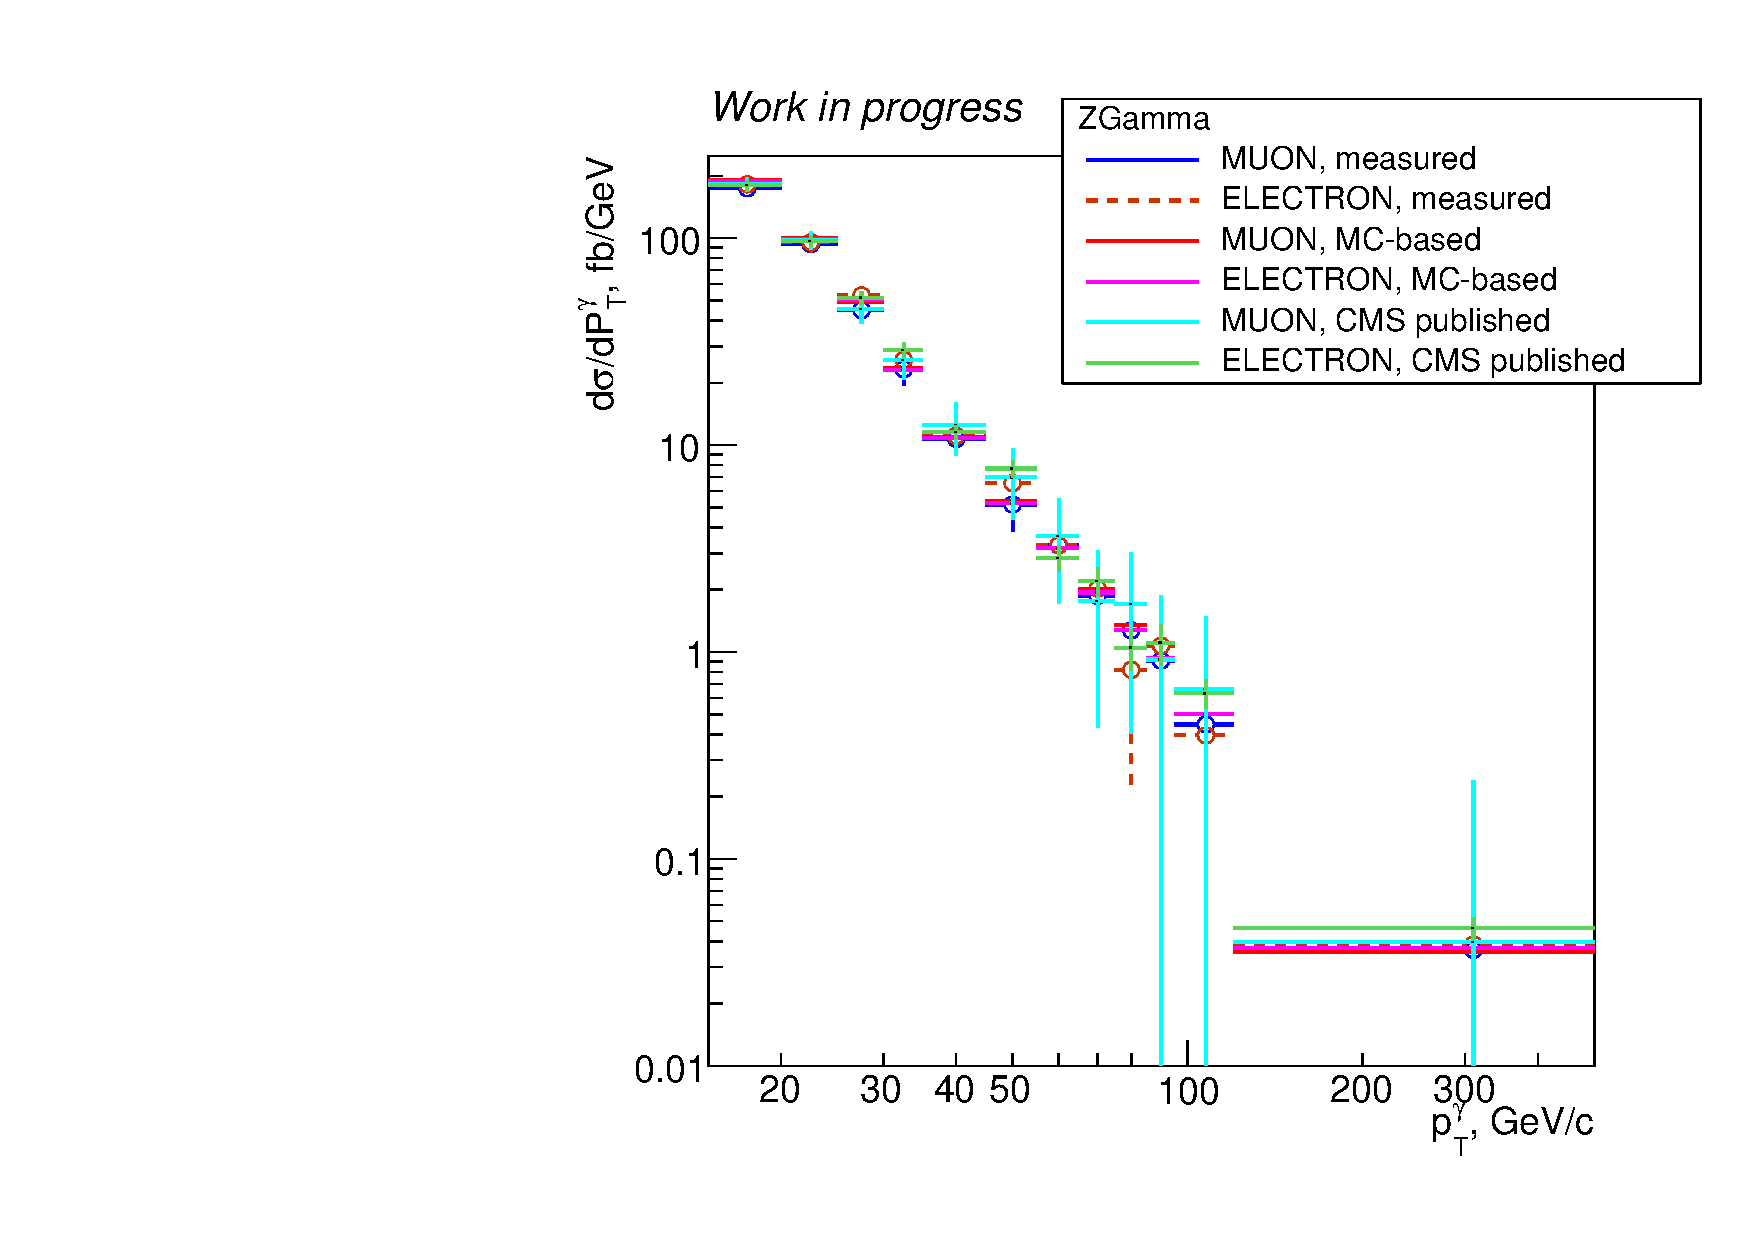
\includegraphics[width=0.45\textwidth]{../figs/figs_v11/ChannelsMERGED_ZGamma/CrossSection/compareCSZGamma.pdf}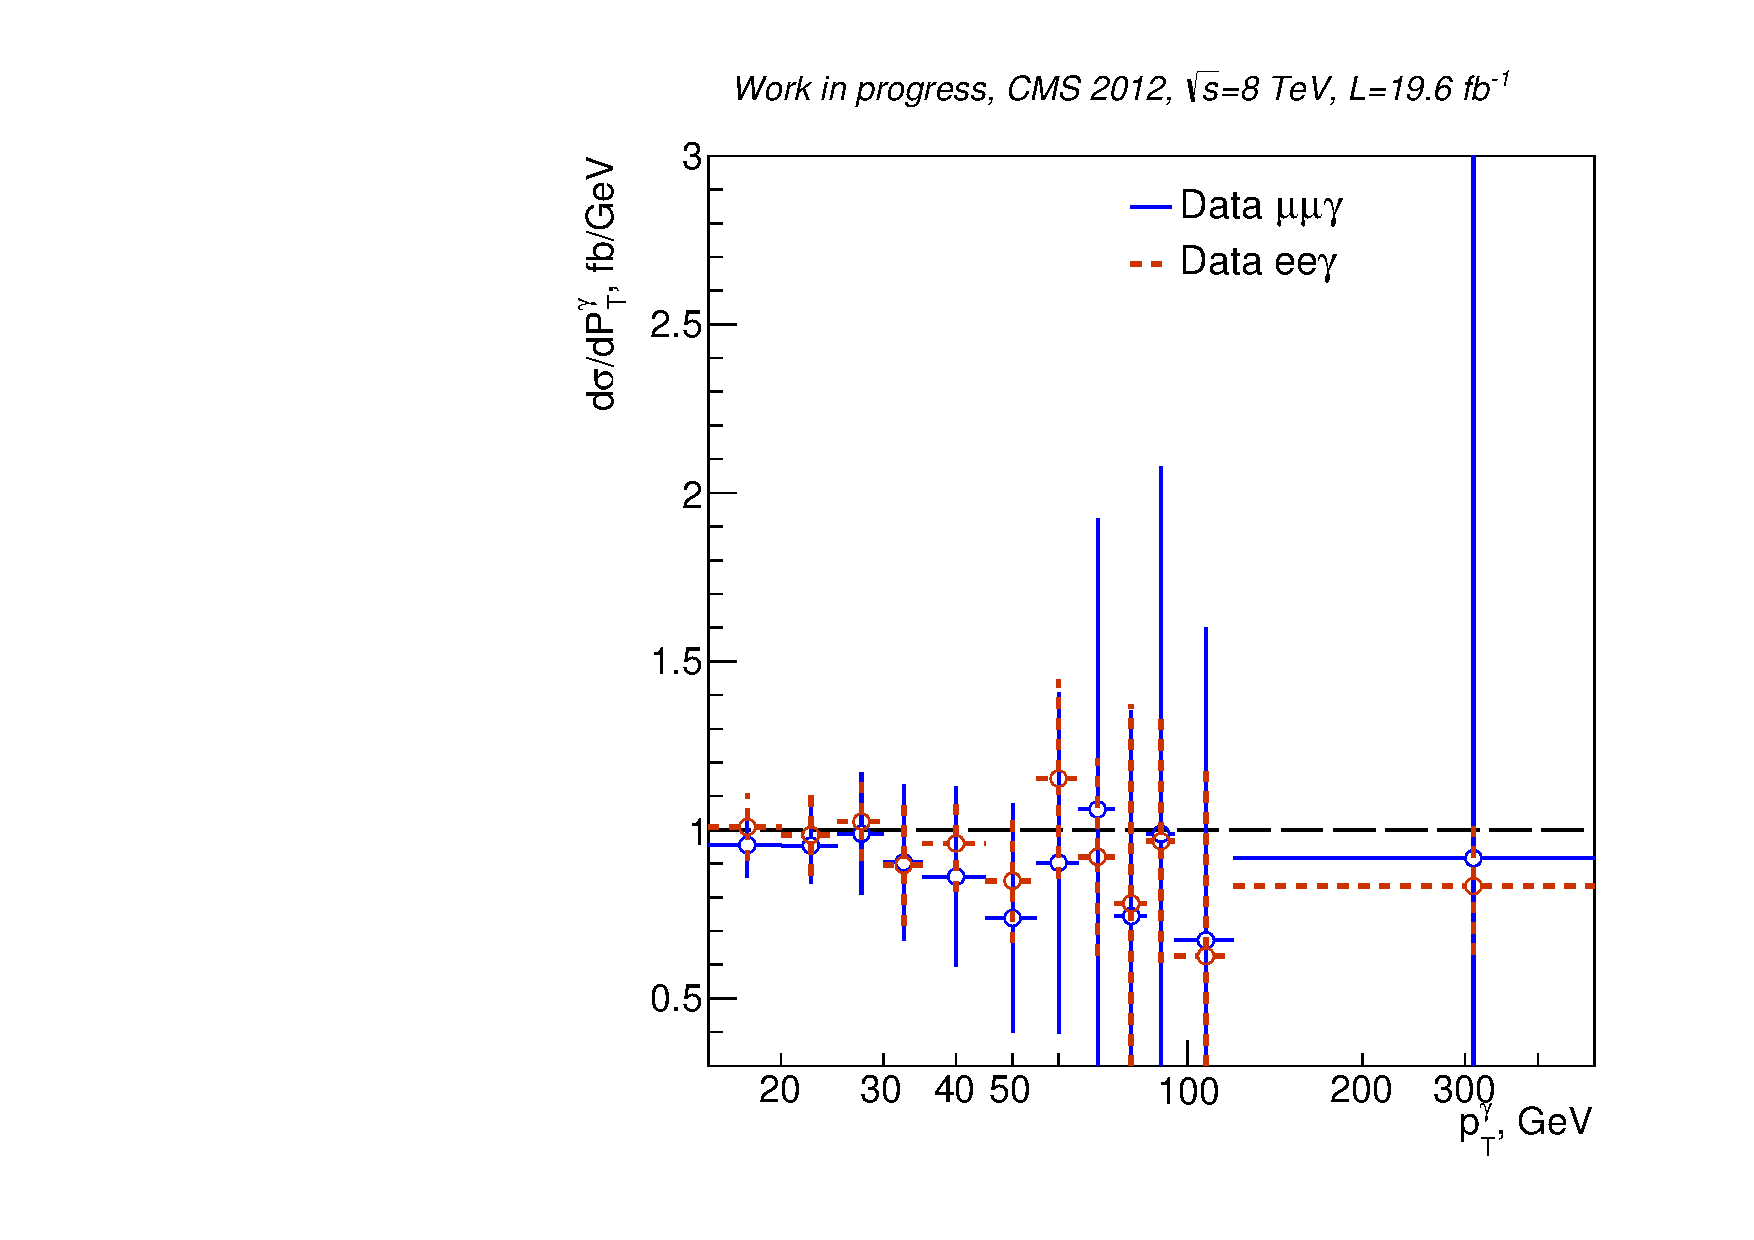
\includegraphics[width=0.45\textwidth]{../figs/figs_v11/ChannelsMERGED_ZGamma/CrossSection/compareCSratioOttoZGamma.pdf}
  \end{center}
\end{figure}
  \tiny
  \begin{itemize}
    \item Total and differential cross section of $Z\gamma\rightarrow ll\gamma$ is measured and agrees well with the 8 TeV published CMS result as well as with the theory prediction;
     \item The workflows for the $Z\gamma$ and $W\gamma$ are very similar, and we used the same procedures of the jets$\rightarrow\gamma$ background estimation;
     \item For the muon channel, data used for preparing templates significantly overlap with the dataset, thus, the result is a closure test rather that a valid physics measurement;
     \item For the electron channel, templates and the dataset are independent, thus, the result is a valid physics measurement. 
  \end{itemize}
\end{frame}%{Differential Cross Section. Plots}
